In order to see when changes were made to a \gdcase{}, \gdsuite{} or \gdjob{} in a \gdproject{}, you can activate the change tracking option in the \gdproject{} properties. 

When this option is activated, each \gdcase{}, \gdsuite{} and \gdjob{} shows information on the timestamp of a change, and the type of change (created or modified). You can optionally enter a property which should be displayed alongside the change type to track e.g. the user that made the change. The changes that lead to change information being shown are:
\begin{itemize}
\item The creation of a node.
\item Any time an editor is saved (renaming within an editor, adding \gdcases{} to an editor, removing \gdcases{} from an editor, adding data or component names, using the refactor actions from within an editor. 
\end{itemize}
\gdproject{}-wide refactor actions, such as those started from the search result view, and any renaming in browsers, are not shown in the change information. 

\subsubsection{Activating change tracking}

\begin{enumerate}
\item Open the \gdproject{} properties:\\
\bxmenu{Test}{Properties}{}\\
\item Select \bxname{General} from the tree on the left-hand side.
\item Activate \bxname{Track changes} to activate change tracking for this \gdproject{}. 
\item Choose whether you want to track a certain number of changes per node, or whether you want to keep changes for a specific time span. Enter the amount of changes or days. 
\bxtipp{The display for each node is updated on saving. If there are too many changes, or some changes are outside of the specified time span, they will be removed on saving.}
\item You can (optionally) enter a system or environment property that is displayed in the \gdpropview{} as additional information about the change (e.g. the user that made the change).
\end{enumerate}
 When change tracking is activated, the \gdpropview{} for the original specification (not places of reuse) for \gdcases{}, \gdsuites{} and \gdjobs{} displays information on the changes made \bxfigref{TasksTrackChangesPropView}. 

\begin{figure}[h]
\begin{center}
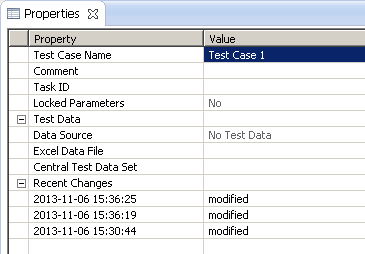
\includegraphics{Tasks/Projects/PS/ChangeTrackingPropView}
\caption{Tracking Changes}
\label{TasksTrackChangesPropView}
\end{center}
\end{figure}

You can deactivate change tracking via the \gdproject{} properties. To remove all current information about changes, use the \bxname{delete} option \bxpref{TasksRemoveChangeTracking}.

\subsubsection{Removing change tracking information from a \gdproject}
\label{TasksRemoveChangeTracking}
\begin{enumerate}
\item To remove all information on all nodes about changes made, open the \gdproject{} properties:\\
\bxmenu{Test}{Properties}{}\\
\item Select \bxname{General} from the tree on the left-hand side.
\item Click the button \bxcaption{Delete all tracked data} and confirm when asked. 
\item All data will be removed from the \gdproject{} that were collected for the change tracking. 
\bxwarn{If a node is currently locked, then the data for this node will not be removed. You will see which nodes are affected in a dialog. We recommend deleting change tracking data when you are sure that no one else is using the \gdproject{}.}
\end{enumerate}
